\documentclass[border=10pt]{standalone}
\usepackage{tikz}
\usepackage{array}
\usepackage{colortbl}
\usepackage{booktabs}

\definecolor{darkblue}{RGB}{0,51,102}
\definecolor{lightblue}{RGB}{230,242,255}

\begin{document}

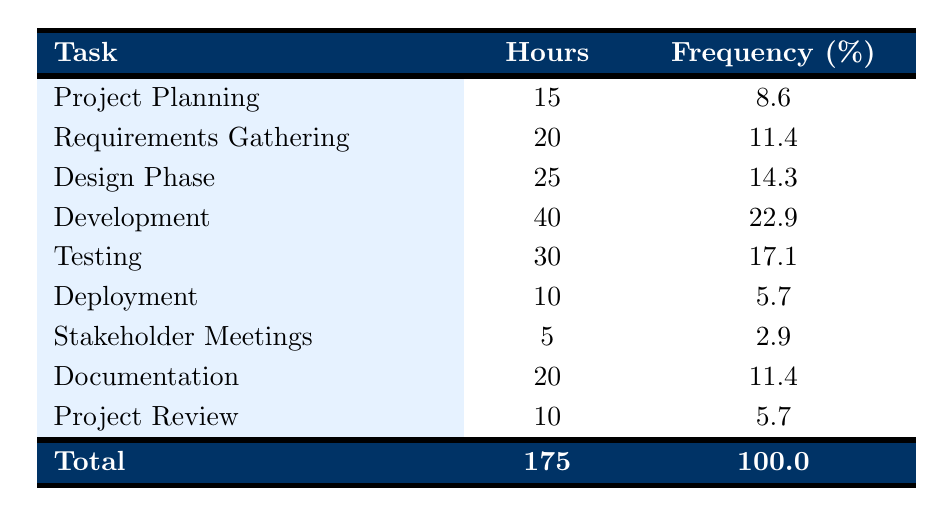
\begin{tikzpicture}
    % Define the table using a node with tabular content
    \node[inner sep=0pt] at (0,0) {
        \renewcommand{\arraystretch}{1.2}
        \begin{tabular}{>{\raggedright\arraybackslash}p{5cm}>{\centering\arraybackslash}p{1.7cm}>{\centering\arraybackslash}p{3.2cm}}
            \noalign{\hrule height 2pt}
            \rowcolor{darkblue}
            \textcolor{white}{\bfseries Task} & 
            \textcolor{white}{\bfseries Hours} & 
            \textcolor{white}{\bfseries Frequency (\%)} \\
            \noalign{\hrule height 2pt}
            \cellcolor{lightblue}Project Planning & 15 & 8.6 \\
            \cellcolor{lightblue}Requirements Gathering & 20 & 11.4 \\
            \cellcolor{lightblue}Design Phase & 25 & 14.3 \\
            \cellcolor{lightblue}Development & 40 & 22.9 \\
            \cellcolor{lightblue}Testing & 30 & 17.1 \\
            \cellcolor{lightblue}Deployment & 10 & 5.7 \\
            \cellcolor{lightblue}Stakeholder Meetings & 5 & 2.9 \\
            \cellcolor{lightblue}Documentation & 20 & 11.4 \\
            \cellcolor{lightblue}Project Review & 10 & 5.7 \\
            \noalign{\hrule height 2pt}
            \rowcolor{darkblue}
            \textcolor{white}{\bfseries Total} & 
            \textcolor{white}{\bfseries 175} & 
            \textcolor{white}{\bfseries 100.0} \\
            \noalign{\hrule height 2pt}
        \end{tabular}
    };
\end{tikzpicture}

\end{document}
